\documentclass{article}
\usepackage{tikz}
\usetikzlibrary{automata,positioning}

\begin{document}

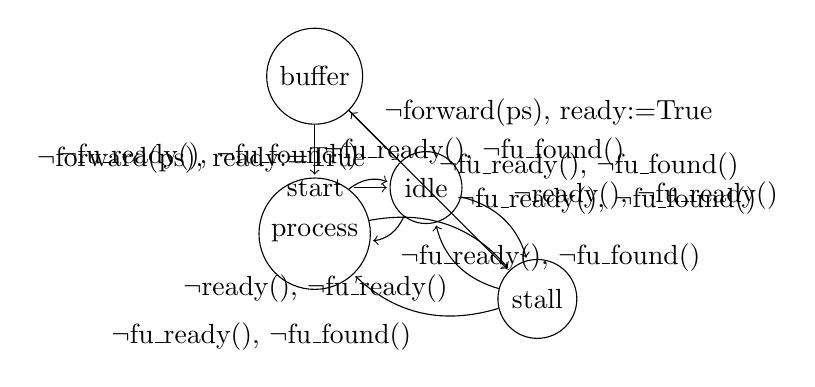
\begin{tikzpicture}[shorten >=1pt,node distance=2cm,on grid,auto]
    \node[state,initial] (idle) {idle};
    \node[state,above left=of idle] (buffer) {buffer};
    \node[state,below right=of idle] (stall) {stall};
    \node[state,below=of buffer] (process) {process};

    \path[->]
    (idle) edge node {$\neg$forward(ps), ready:=True} (buffer)
    (idle) edge[bend left] node {$\neg$ready(), $\neg$fu\_ready()} (stall)
    (idle) edge[bend left] node {$\neg$fu\_ready(), $\neg$fu\_found()} (process)
    (buffer) edge node {$\neg$forward(ps), ready:=True} (idle)
    (buffer) edge node {$\neg$fu\_ready(), $\neg$fu\_found()} (stall)
    (buffer) edge node {$\neg$fu\_ready(), $\neg$fu\_found()} (process)
    (stall) edge[bend left] node {$\neg$ready(), $\neg$fu\_ready()} (idle)
    (stall) edge[bend left] node {$\neg$fu\_ready(), $\neg$fu\_found()} (process)
    (process) edge[bend left] node {$\neg$fu\_ready(), $\neg$fu\_found()} (idle)
    (process) edge[bend left] node {$\neg$fu\_ready(), $\neg$fu\_found()} (stall)
    ;
\end{tikzpicture}

\caption{State diagram of the ACADL ExecuteStage class, where \texttt{fu} represents any of the contained FunctionalUnits, and \texttt{ps} represents any of the connected PipelineStages.}
\label{fig:execute_state_diagram}

\end{document}